\documentclass[a4paper]{article}

\usepackage[utf8]{inputenc}
\usepackage[T1]{fontenc}
\usepackage{textcomp}
\usepackage{amsmath, amssymb, amsthm}

\usepackage{setspace}
\usepackage{tikz}

\usetikzlibrary{automata, arrows, chains}
\tikzset{
	>=stealth, % makes the arrow heads bold
	node distance=3cm, % specifies the minimum distance between two nodes. Change if necessary.
	every state/.style={thick, fill=gray!10}, % sets the properties for each ’state’ node
	initial text=$ $, % sets the text that appears on the start arrow
	in place/.style={
		auto=false,
		inner sep=3pt,
	},
}

% figure support
\usepackage{import}
\usepackage{xifthen}
\pdfminorversion=7
\usepackage{pdfpages}
\usepackage{transparent}
\newcommand{\incfig}[1]{%
	\def\svgwidth{\columnwidth}
	\import{./figures/}{#1.pdf_tex}
}

\pdfsuppresswarningpagegroup=1

\title{Stat2 HW: Data Cleaning}
\date{Sep 14, 2022}
\author{Jack Ruder}


\begin{document}

\doublespacing
\maketitle

\section*{1}
We see that there are 123 variables in the data.

\section*{2}
There are 3901 rows/observations in the data.

\section*{3}%
We can aggregate count all of the NA entries, in the Head Length column there are 2600 empty values.

\section*{4}%
The correct units are \(\dfrac{\textnormal{Years}}{1000}\), scaling the age range to 2.001 to 20.054 years, consistent with the study. Dividing the Age in Months column by the age in Years Colmun yields an average ratio of \(\frac{1}{12}\), so these units must be correct.

\section*{5}%
From the pdf on pages 454 and 461, we observe that the min weight is 10.2kg, and the max weight is 112.3kg, within the age ranges present in the data.
The range in the data is 10 times these numbers, so clearly the weight is in units of \(\frac{\textnormal{kg}}{10}\).

\section*{6}%
In the text on page 41, it is described that Males are assigned a 1 in the data, and Females are assigned a 2. We check that this is accurate in the data set by
looking at average weights of males compared to females for ages older than 17, and we see that those with a 1 assigned in the gender column are heavier as expected. 

\section*{7, 8, 9}%
Here, there are 5 values shown in the table. 309 enteries are neither 1 nor 2. In the pdf, a questionnaire provides Right Handed, Left Handed, and Both as options. Since 1 has by far the most entries, and it is listed first on the form, it is a logical choice for Right handed. 2 has the next most, so it is probably Left handed. This numbering is consistent with the assignment of Male and Female. A value of 3 lakes sense to be Both following the rationale for 1 and 2. 0 and 5 are the strange values, and lack any description in the pdf. From page 41, we know that the data was entered by humans using words, and transcribed in software to a number. 0 Likely then means N/A of sorts(missing values), since none of the values in the Handedness column are N/A. Looking at the single entry for 5, it is hard to see any pattern for why there exists a unique value. Potentially 5 represents a disability of sorts, although there is no comment code for the entry.

\section*{10}%
As described by page 75 of the pdf, stature records the height measured by the distance from the floor to the top of the subjects head.
Again, it seems that units in the table are scaled by 10, likely to maintain precision in absence of float/double datatypes. Units then in this column are \(\frac{\textnormal{cm}}{10}\), or mm.

\section*{11}%
\label{sec:11}

The questionnaire on pg. 28 of the pdf describes the birth order as the order in which children were born, with 1 being the oldest, 2 being the second oldest, and so on.
The values that are most questionable in this column are 0, 20 and 90. 
In consistency with the handedness column the most likely scenario is that 0 is for a blank. Being the 20th born while unlikely seems plausible, so we will make the assumption that somebody has 19 previous siblings. It seems that 90 must be a computer assigned code. Potentially this value represents that the field was filled out as unknown by the subject, but not left blank.

\section*{12}
\begin{figure}[htpb]
	\centering
	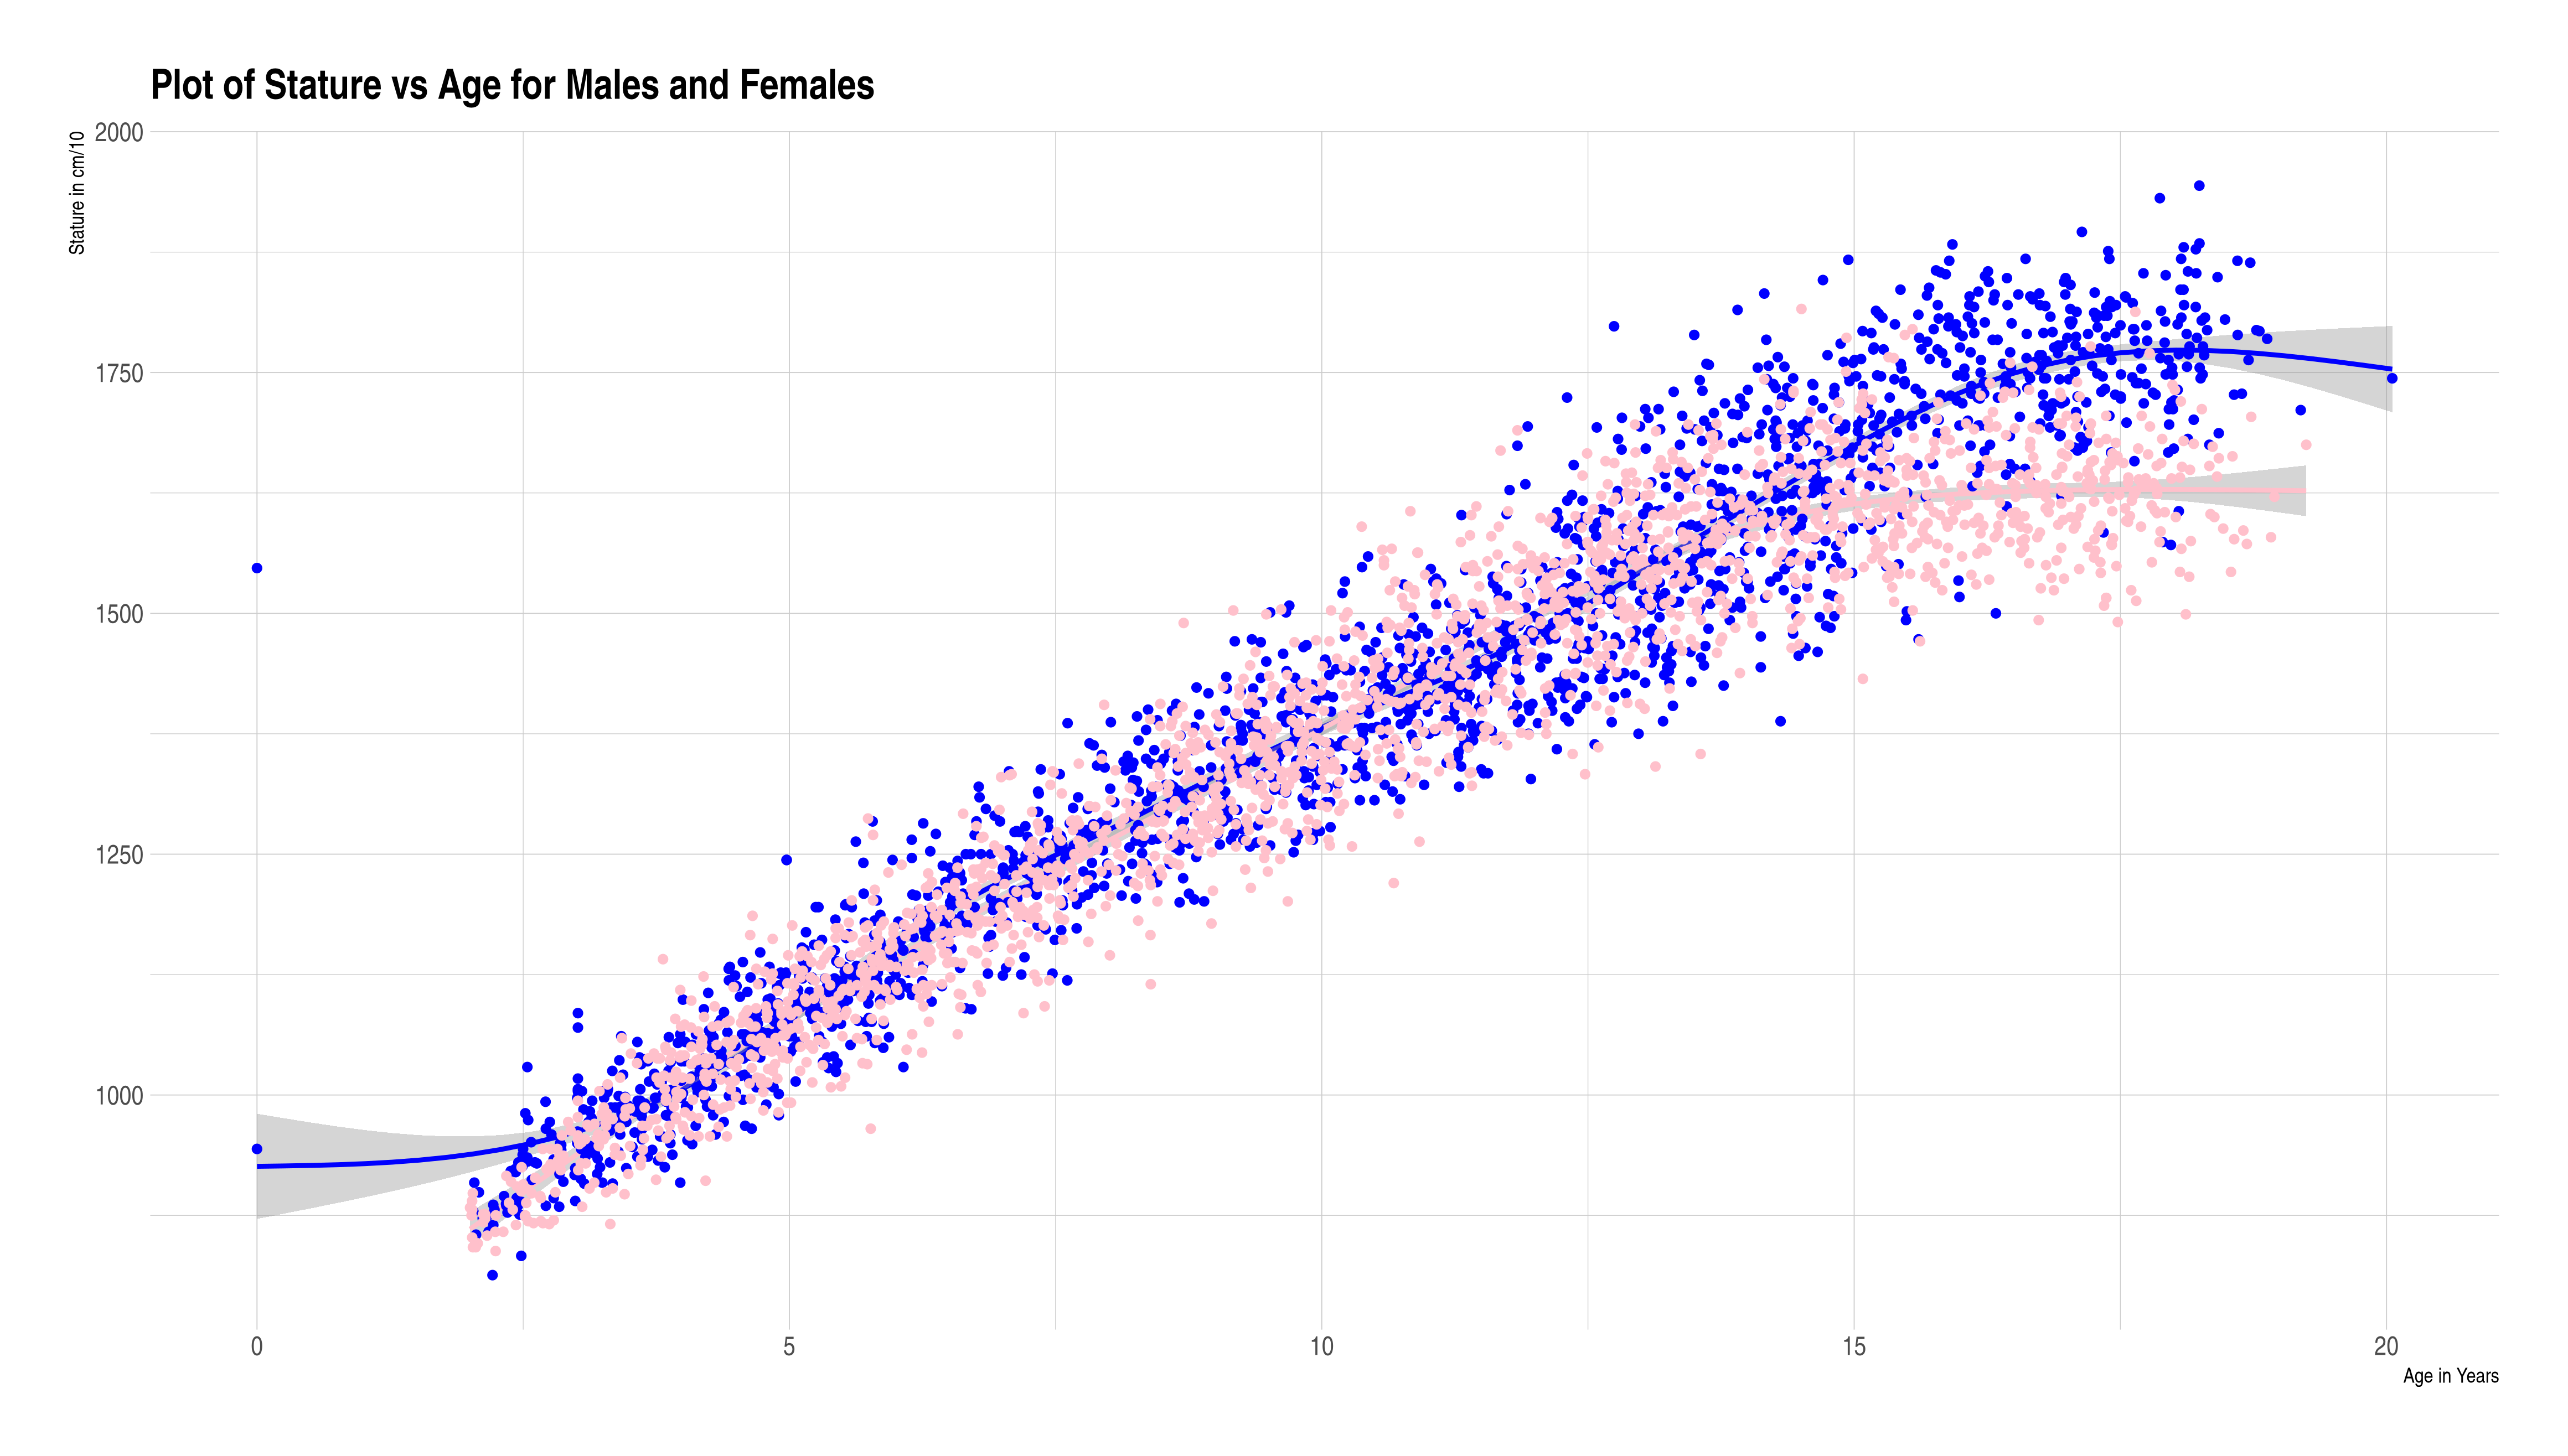
\includegraphics[width=\textwidth]{q12.png}
	\caption{Males in Blue, Females in Pink}
\end{figure}

\section*{13}%
\label{sec:13}
Viewing the histogram of upper arm circumferences, we see a definite skew to the right. Performing a log transform yields a normal looking distribution, with a wide peak and short tails.
\end{document}
